\section{Vehicle Actuated Programming in Vissim}
\label{vap}
VAP is an optional module for Vissim which enables direct programming of signal controllers. VAP is a simple, label-based (goto) language. The main feature is access to a library of functions, which manipulate the state of the signal controller. 

With VAP there is a graphical program, VISVAP, that allows the user to design a flow-chart description of the controller logic, rather than writing it in VAP, as VISVAP can compile the flow-chart into VAP. Figure \ref{fig:visvap_example} shows an example of a simple logic to control the lights at the ring 3 / Herlev Sygehus intersection.

\begin{figure}[!ht]
\begin{center}
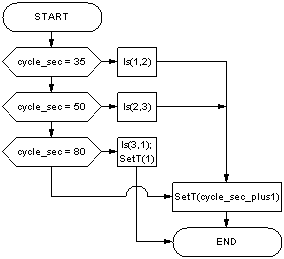
\includegraphics[scale=0.5]{visvap_example_herlev-sygehus.png} 
\end{center}
\caption{VISVAP flow-chart description of simple fixed-time logic for Herlev Sygehus / ring 3}
\label{fig:visvap_example}
\end{figure}

The VAP program is called once for every simulation second. The starting label is START and the program proceeds as indicated by the arrows until the END label has been reached. Diamond boxes are logical tests where the right-going arrow indicates TRUE and down-going indicates FALSE. Square boxes contain expressions, in this case we use \verb|Is(<stage_from>,<stage_to>)| to switch between stages, when a certain portion of the current cycle time has passed. Below is the VAP code, which corresponds to the flow-chart:

\begin{verbatim}
/* EXPRESSIONS */ 
            cycle_sec := T;
            cycle_sec_plus1 := cycle_sec + 1;

/* MAIN PROGRAM */ 

S00Z001:    IF cycle_sec = 35 THEN
S01Z001:      Is(1,2)
            ELSE
S00Z002:      IF cycle_sec = 50 THEN
S01Z002:        Is(2,3)
              ELSE
S00Z003:        IF cycle_sec = 80 THEN
S01Z003:          Is(3,1); SetT(1);
                  GOTO PROG_ENDE
                END
              END
            END;
S02Z004:    SetT(cycle_sec_plus1)
PROG_ENDE:    .
\end{verbatim}

VAP is unsuited for complex controller logic, such as ones involving predictions and optimization by iteration. This is due to the fact that VAP only has support for basic programming language constructs and the label-based nature of the language, which is detrimental to larger code bases see eg. the statement by Dijkstra \cite{nogoto}. As an example the above VAP code could be simplified into:

\begin{verbatim}
switch(T){
case 35: Is(1,2); SetT(T+1)
case 50: Is(2,3); SetT(T+1)
case 80: Is(3,1); SetT(1)
case else:  /* do nothing */
}
\end{verbatim}

VAP is suitable, however, for implementation of DOGS due to its simple decision system as described in section \ref{dogs}. In this section I will describe how the DOGS logic was implementated in VAP.

\subsection{DOGS}
